\documentclass[10pt,conference]{IEEEtran}
\usepackage{graphicx,booktabs,url}
\usepackage[T1]{fontenc}
\usepackage[utf8]{inputenc}
\begin{document}
\title{Benchmarking Human-Written and LLM-Generated TypeScript Projects: Milestone Progress Report}
\author{\IEEEauthorblockN{Simon Xie, Sukhdip Kandola, Thang To}\IEEEauthorblockA{CMPT 479 D100, School of Computing Science, Simon Fraser University, Burnaby, BC, Canada}}
\maketitle

\begin{abstract}
This milestone report documents our progress on an empirical benchmark that compares human-written and LLM-generated TypeScript projects. We have (i) built an automated, Docker-isolated pipeline. It clones each repository at a pinned commit, installs it from its own lockfile, and measures compilation (\texttt{tsc}), code quality (ESLint with typescript-eslint and SonarSource rules), maintainability (cyclomatic and cognitive complexity, duplication, comment density) and test effectiveness (the project's own tests and StrykerJS mutation testing). (ii) We assembled a size-matched dataset of 12 human-written repositories pinned before 2021 and 12 agent-built repositories, whose authorship we verify from AI co-author commit trailers. (iii) We ran the pipeline on all 24 repositories. In preliminary results, the LLM group has far fewer lint violations per KLOC (median 42.8 vs. 7.6) but more complex functions (mean cyclomatic complexity 1.96 vs. 2.85). Its own test suites also pass more often on a current Node.js (8/12 vs. 5/12), largely because old human suites have decayed. We found no significant difference in duplication, comment density, test-to-code ratio or compiler errors. The report ends with the remaining work toward the final paper.
\end{abstract}
\begin{IEEEkeywords}
LLM-generated code, TypeScript, empirical software engineering, static analysis, mutation testing, benchmark
\end{IEEEkeywords}

\section{Introduction}
LLM coding agents such as Claude Code, Cursor and Codex now write entire repositories, not just snippets. Code that compiles and looks plausible may still hide defects, poor practices or weak tests. Prior comparisons of human and LLM code study Python or Java \emph{functions} generated for benchmark tasks [2]--[4]. We instead compare \emph{whole, real-world TypeScript projects} published on GitHub, in an ecosystem with its own characteristic failure modes [1]. Our research questions are unchanged from the proposal:

\begin{itemize}
\item \textbf{RQ1} How does code quality differ between human-written and LLM-generated TypeScript projects?
\item \textbf{RQ2} How do complexity, maintainability and structural testability differ?
\item \textbf{RQ3} Do LLM-generated projects have more compilation errors?
\end{itemize}

Since the proposal (Oct.~19) and the literature review (Nov.~2), we have completed the dataset-collection and infrastructure phases of our plan and a first full evaluation run. Table~I gives the status of each phase. The rest of this report covers the dataset (Sec.~II), the pipeline (Sec.~III), preliminary results (Sec.~IV), threats to validity (Sec.~V) and remaining work (Sec.~VI).

\begin{table}[t]
\caption{Progress against the project plan}
\label{tab:progress}
\centering
\scriptsize
\setlength{\tabcolsep}{2.5pt}
\begin{tabular}{lcc}
\toprule
Phase (from proposal) & Status & Evidence \\
\midrule
1. Literature review and design & Done & Review (Nov. 2); design refined (Sec. II--III) \\
2. Dataset collection & Done & 1236 candidates $\rightarrow$ 12+12 repos, frozen SHAs \\
3. Infrastructure & Done & Dockerized pipeline, open-source repository \\
4. Evaluation & First full run done & All 24 repos, all stages \\
5. Analysis and reporting & In progress & Preliminary statistics (Sec. IV) \\
\bottomrule
\end{tabular}
\end{table}

\section{Dataset Construction}
\subsection{Discovery and screening}
Candidates come from the GitHub search API (\texttt{bench/discover.py}). Human candidates are TypeScript repositories created between 2016 and mid-2020, with 100--3,000 stars and no push after 2021. LLM candidates are TypeScript repositories created in 2025 or later whose README advertises agent-built development (“built with Claude Code”, “vibe coded”, “built with Codex”, ...). This yielded 1236 unique candidates (222 human, 1014 LLM). A screening stage (\texttt{bench/screen.py}) fetches each repository's root \texttt{package.json}, \texttt{tsconfig.json}, language breakdown and latest 100 commits with batched GraphQL queries. It then applies fixed eligibility rules: a root package and tsconfig, a real \texttt{test} script (vitest, jest, mocha, ava, jasmine or \texttt{node --test}), no workspaces, $\geq$60\% TypeScript, and 40~KB--1.5~MB of TypeScript. 72 human and 34 LLM repositories were eligible. Every decision and its reason is recorded in \texttt{dataset/screened.csv}.

\subsection{Verifying authorship}
The proposal classified projects by release date alone, which is unreliable. For the LLM group we now require \emph{positive evidence}. Coding agents leave machine-readable traces in commit metadata, such as Claude Code's \texttt{Co-Authored-By: Claude} trailer, Cursor, Copilot and Codex co-author trailers, and agent bot authors. \texttt{bench/authorship.py} detects ten such agents. An LLM repository is eligible only if $\geq$50\% of its latest 100 commits carry such a trailer. This removed 779 of the 1014 self-described LLM candidates, so README claims alone would have mislabelled most projects. After cloning, the share is recomputed over the full history. The selected LLM repositories have a median of 75\% agent-attributed commits (range 27--100\%), from claude-code, codex, cursor, devin. This is a lower bound, since agents can be used without trailers. For the human group we keep a date rule but make it airtight. Each repository is \emph{pinned to its last commit before 2021-01-01}, which predates GitHub Copilot's preview (June 2021) and ChatGPT (Nov. 2022). None of their commits carry an agent trailer.

\subsection{Selection and matching}
Selection is deterministic (\texttt{bench/select\_repos.py}). We take the 12 most-starred eligible LLM repositories and pair each with the not-yet-chosen eligible human repository ($\geq$100 stars) closest in TypeScript size on a log scale. Twelve per group exceeds the proposal's target of ten, which leaves spares if a project cannot be analysed. Table~II lists the frozen dataset. Production code ranges from 0.5 to 17.0 KLOC (median 6.1 human vs. 7.8 LLM), and the analysed commit SHAs are in \texttt{dataset/repos.csv}.

\begin{table}[t]
\caption{Benchmarked repositories (KLOC: production code; Test: test-code KLOC; AI\%: agent-attributed commits up to the pin)}
\label{tab:dataset}
\centering
\scriptsize
\setlength{\tabcolsep}{2.5pt}
\begin{tabular}{lccccc}
\toprule
ID & Repository & Pin date & KLOC & Test & AI\% \\
\midrule
H01 & Lucifier129/bistate & 2020-07-24 & 0.5 & 1.6 & 0 \\
H02 & ionic-team/ionic-app-scripts & 2020-04-30 & 8.7 & 5.9 & 0 \\
H03 & helios1138/graphql-typed-client & 2020-01-23 & 1.4 & 1.1 & 0 \\
H04 & HadoukenIO/core & 2019-10-17 & 12.4 & 1.6 & 0 \\
H05 & HSEIreland/covid-tracker-app & 2020-10-01 & 17.0 & 0.0 & 0 \\
H06 & microsoft/vscode-chrome-debug-core & 2020-08-23 & 6.5 & 3.5 & 0 \\
H07 & yuche/gouqi & 2017-06-13 & 11.1 & 3.8 & 0 \\
H08 & monicahq/old\_mobile\_app & 2018-09-22 & 6.2 & 6.5 & 0 \\
H09 & tsukhu/nxplorerjs-microservice-starter & 2020-02-03 & 3.6 & 0.3 & 0 \\
H10 & r-park/soundcloud-ngrx & 2017-07-02 & 2.5 & 3.8 & 0 \\
H11 & hastic-zzz/hastic-grafana-app & 2020-12-26 & 4.2 & 0.1 & 0 \\
H12 & samuelmeuli/mini-diary & 2020-05-29 & 6.0 & 0.1 & 0 \\
L01 & tamaratran/fast-jev-compaction & 2026-09-17 & 1.1 & 0.5 & 97 \\
L02 & UfoMiao/zcf & 2026-10-29 & 11.1 & 8.7 & 27 \\
L03 & hoquanghai/Auto-Create-Video & 2026-05-02 & 1.3 & 0.5 & 76 \\
L04 & agent-era/devteam & 2026-05-25 & 14.0 & 14.2 & 44 \\
L05 & mcollina/githuman & 2026-04-12 & 14.2 & 9.9 & 83 \\
L06 & maksutovic/joycraft & 2026-11-03 & 8.5 & 19.4 & 65 \\
L07 & prodlint/prodlint & 2026-11-01 & 7.2 & 9.4 & 98 \\
L08 & Sqcows/forgejo-mcp & 2026-10-15 & 10.2 & 3.6 & 95 \\
L09 & roboco-io/roboco-cli & 2026-05-06 & 2.4 & 1.3 & 58 \\
L10 & menagerai/menagerai & 2026-11-07 & 4.8 & 3.5 & 51 \\
L11 & andrisasuke/podlogs & 2026-10-22 & 3.4 & 0.3 & 73 \\
L12 & cjy20040604-hub/eyes-training & 2026-10-18 & 15.2 & 6.8 & 100 \\
\bottomrule
\end{tabular}
\end{table}

\section{Benchmark Infrastructure}
The pipeline follows the proposed design (retrieve $\rightarrow$ install $\rightarrow$ build and test $\rightarrow$ collect) and is fully automated in Python (\texttt{bench/run.py}). Each repository is cloned on the host without blobs and checked out at its pin, with line-ending conversion disabled. It is then copied into a \emph{fresh container} built from our image (Node~22 plus the pinned toolchain). The host copy is mounted read-only and the container is discarded afterwards, so install scripts, tests and mutants never touch the host. Stages are resumable, and all raw artefacts are kept per repository. The stages are:

\begin{itemize}
\item \textbf{Inventory and size.} \texttt{.ts}/\texttt{.tsx} files are split into production and test code by \texttt{*.test}/\texttt{*.spec} names and test directories. Build output, declaration files, configuration and tooling scripts are excluded. Code and comment lines are counted with the TypeScript parser, using SonarQube's definitions.
\item \textbf{Code quality (RQ1).} Every project gets one ESLint~9 configuration (\texttt{@eslint/js}, typescript-eslint and SonarJS recommended rules), and the project's own \texttt{eslint-disable} comments are ignored. Each violation is typed by its rule's \texttt{meta.type}: \emph{problem} (likely bug) or \emph{suggestion}.
\item \textbf{Maintainability (RQ2).} Per-function cyclomatic [8] and cognitive [9] complexity (ESLint \texttt{complexity} and SonarJS \texttt{cognitive-complexity}, threshold 0), duplication via jscpd (100-token / 5-line minimum, as in SonarQube), and comment density.
\item \textbf{Compilation (RQ3).} Dependencies are installed with the project's own package manager and lockfile (npm, yarn or pnpm via Corepack), with logged fallbacks. The project's \emph{own} TypeScript version then runs against its own \texttt{tsconfig.json}, including referenced sub-projects. Diagnostics are counted by \texttt{TS} code, separately for project files and for dependencies.
\item \textbf{Tests and mutation (RQ2).} The project's \texttt{test} script runs with a 15-minute limit. When it passes, StrykerJS~10 [7], [12] mutates a seeded random sample of production files (about 400 lines, at most 10 files). It uses the native vitest, jest or mocha runner where the framework version allows, and the command runner otherwise. Stryker is pre-installed in the image so that it never re-resolves the project's dependency tree. Suites that fail on Node~22 are re-run on a Node version from their own era (8--14, taken from \texttt{.nvmrc}, \texttt{engines} or the pin date) to separate broken tests from environment drift.
\end{itemize}

One deliberate change from the proposal: instead of operating a SonarQube server, we run SonarSource's JavaScript/TypeScript analyzer rules (SonarJS, the engine inside SonarQube) through ESLint, plus SonarQube-equivalent duplication and comment metrics. This gives the same per-rule and per-function measurements without a stateful server, and every run is reproducible from a single Docker image.

\section{Preliminary Results}
All 24 repositories completed every static stage. Group differences are tested with two-sided Mann--Whitney U tests. Effect sizes are Cliff's~$\delta$ (positive means higher in the LLM group; magnitudes follow [10]), and \emph{p}-values are Holm-corrected [11] across the 18 metrics in Table~III. With 12 projects per group the results are exploratory. Fig.~1 shows the per-project distributions of six key metrics.

\begin{figure}[t]
\centering
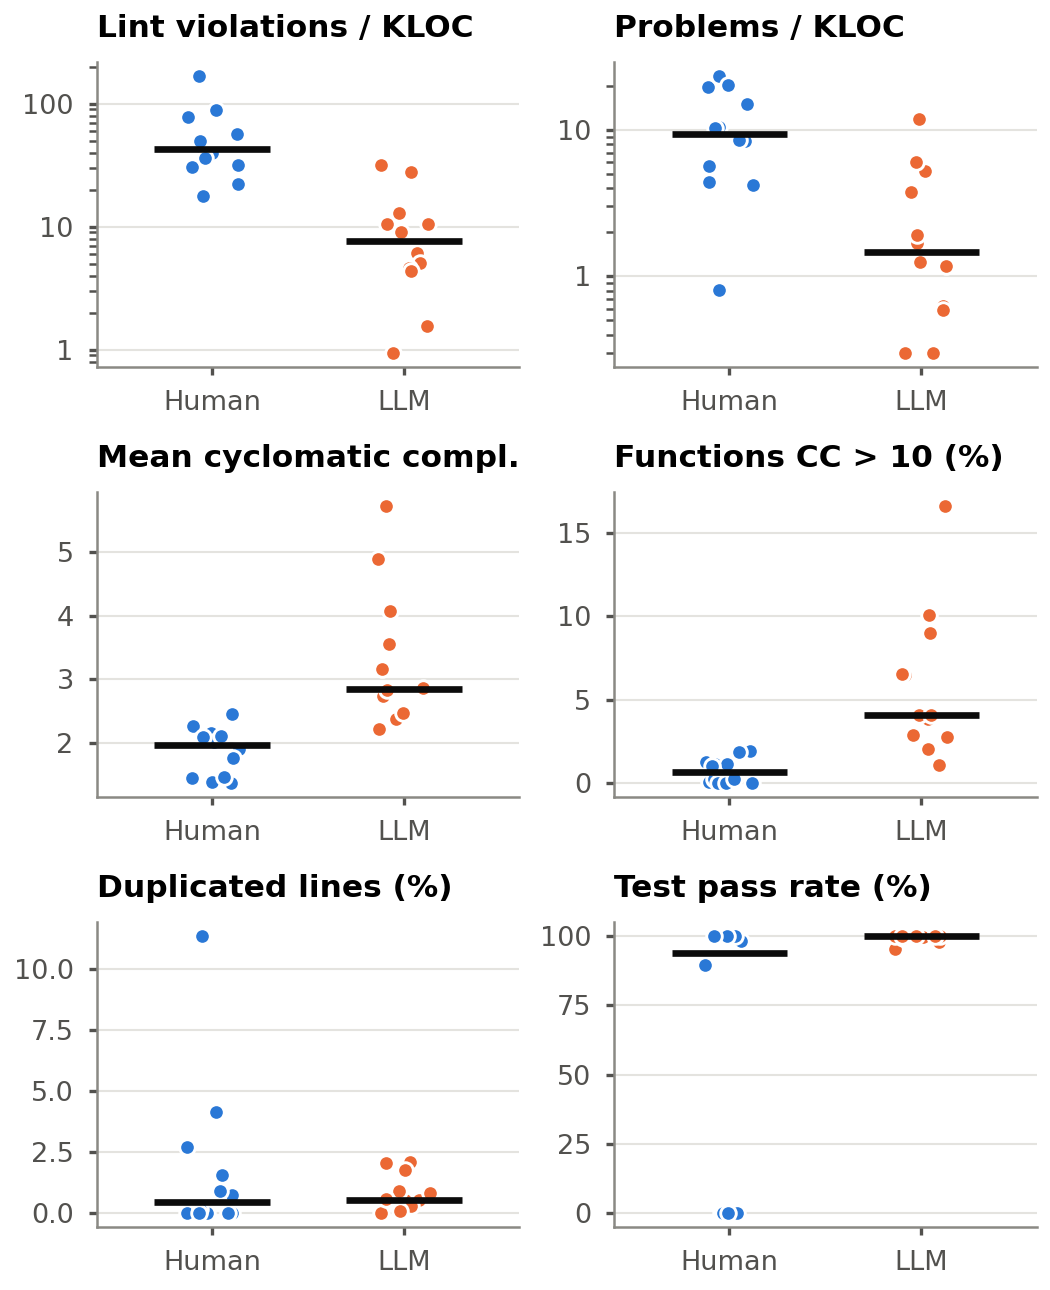
\includegraphics[width=\columnwidth]{figures/metrics_by_group.png}
\caption{Per-repository values by group (dots) and group medians (bars). Violation panels use a log axis, with zero-violation projects drawn at the axis floor. Suites that could not run count as 0\% passing.}
\label{fig:metrics}
\end{figure}

\begin{table}[t]
\caption{Group medians and tests ($\delta$: Cliff's delta, LLM vs. human)}
\label{tab:stats}
\centering
\scriptsize
\setlength{\tabcolsep}{2.5pt}
\begin{tabular}{lcccc}
\toprule
Metric & Human & LLM & $\delta$ & p (Holm) \\
\midrule
Lint violations / KLOC (RQ1) & 42.80 & 7.57 & -0.93 & 0.002 \\
Problem-type violations / KLOC (RQ1) & 9.41 & 1.47 & -0.72 & 0.032 \\
Era-neutral violations / KLOC (RQ1) & 17.46 & 6.03 & -0.51 & 0.281 \\
Explicit \texttt{any} / KLOC (RQ1) & 18.21 & 0.00 & -0.92 & 0.002 \\
Mean cyclomatic complexity / function (RQ2) & 1.96 & 2.85 & +0.96 & 0.002 \\
\% functions with CC \textgreater{} 10 (RQ2) & 0.62 & 4.09 & +0.93 & 0.002 \\
Mean cognitive complexity / function (RQ2) & 1.09 & 1.65 & +0.81 & 0.011 \\
\% functions with cognitive \textgreater{} 15 (RQ2) & 0.23 & 1.70 & +0.83 & 0.008 \\
Functions / KLOC (RQ2) & 115.85 & 76.60 & -0.60 & 0.141 \\
Duplicated lines (\%) (RQ2) & 0.47 & 0.55 & +0.10 & 1.000 \\
Comment density (RQ2) & 0.037 & 0.085 & +0.39 & 0.674 \\
Test-to-code LOC ratio (RQ2) & 0.44 & 0.62 & +0.22 & 1.000 \\
Test pass rate (Node 22) (RQ2) & 0.939 & 1.000 & +0.42 & 0.434 \\
tsc errors in project files / KLOC (RQ3) & 0.00 & 0.00 & -0.03 & 1.000 \\
Mutation score (RQ2) & 0.550 & 0.400 & -0.06 & 1.000 \\
Mutation score, covered code (RQ2) & 0.550 & 0.672 & +0.19 & 1.000 \\
\bottomrule
\end{tabular}
\end{table}

\subsection{RQ1: Code quality}
Contrary to the common expectation that LLM code is of lower quality, the LLM group has fewer lint violations per KLOC (median 42.8 vs. 7.6, Cliff's~$\delta$~=~-0.93 (large), Holm \emph{p}~=~0.002) and fewer \emph{problem}-type violations (median 9.4 vs. 1.5, Cliff's~$\delta$~=~-0.72 (large), Holm \emph{p}~=~0.032). The two groups' rule profiles also differ. Human projects are dominated by \texttt{no-explicit-any}, \texttt{no-unused-vars}, \texttt{no-var}, \texttt{prefer-const}: explicit \texttt{any} alone has a median of 18.2 per KLOC vs. 0.0. LLM projects are dominated by \texttt{no-nested-conditional}, \texttt{cognitive-complexity}, \texttt{no-unused-vars}, \texttt{no-explicit-any}, which are structural rather than typing issues.

Part of this gap is an \emph{era effect}. Older TypeScript lacked \texttt{unknown} (added in 3.0), and code from that time commonly used \texttt{var}, \texttt{require} and wrapper types. Excluding 12 era-dependent rules keeps the direction and a large effect (median 17.5 vs. 6.0, $\delta$~=~-0.51, uncorrected \emph{p}~=~0.035), but the difference is no longer significant after correction (Holm \emph{p}~=~0.281). One plausible contributor is that agents run linters during development and have learned modern typescript-eslint idioms.

\subsection{RQ2: Complexity, maintainability and testability}
The clearest difference runs the other way: LLM-written functions are more complex. Mean cyclomatic complexity is 1.96 vs. 2.85 ($\delta$~=~+0.96, Holm \emph{p}~=~0.002). The share of functions above McCabe's threshold of 10 is 0.6\% vs. 4.1\%, and above Sonar's cognitive threshold of 15 it is 0.2\% vs. 1.7\% ($\delta$~=~+0.83). LLM projects also have fewer functions per KLOC (116 vs. 77, Holm \emph{p}~=~0.141). Together this suggests that agents write fewer, longer, more deeply nested functions, which fits SonarJS's \texttt{no-nested-conditional} being their most frequent violation. Duplication (median 0.47 vs. 0.55, Cliff's~$\delta$~=~+0.10 (negligible), Holm \emph{p}~=~1.000), comment density (median 0.037 vs. 0.085, Cliff's~$\delta$~=~+0.39 (medium), Holm \emph{p}~=~0.674) and test-to-code ratio (median 0.44 vs. 0.62, Cliff's~$\delta$~=~+0.22 (small), Holm \emph{p}~=~1.000) do not differ significantly.

Test runnability differs sharply. The project's own test suite passes on Node~22 for 8 of 12 LLM projects but only 5 of 12 human projects. The per-project pass rate has a median of 93.9\% vs. 100.0\% ($\delta$~=~+0.42, Holm \emph{p}~=~0.434). We diagnosed every failing suite from its logs (\texttt{dataset/test\_failure\_causes.csv}). Re-running the 7 failing human suites on an era-matched Node version made 1 pass (a \texttt{node-sass} binary). Of the remaining human failures, 2 cannot install at all (an unpublished npm package and an unfetchable git dependency), 1 depends on a public API that now returns 403, 1 is a device-only end-to-end suite, and only 2 are genuine failures. The LLM failures are the reverse: 3 of 4 are genuine failing assertions (8 failing tests each, in suites of 372--3,367 tests), and one needs an \texttt{ffmpeg} binary. Human suites mostly \emph{decay}, while LLM suites are committed with a few red tests.

Mutation testing produced a score for 12 of the 13 projects with a passing suite (4263 mutants). The score was median 0.55 (range 0.00--0.82, n~=~4) for human projects and median 0.40 (range 0.09--0.83, n~=~8) for LLM projects; survived and uncovered mutants both count as not killed. Restricted to mutants that some test executes, the medians are 0.55 (human) and 0.67 (LLM). Projects run with the framework-agnostic command runner cannot report coverage, so all their mutants count as covered. We also exclude one project whose tests run against precompiled JavaScript, which mutated TypeScript sources never reach (\texttt{dataset/mutation\_exclusions.csv}). Mutation testing can only run where the tests pass today, so the human sample is small and biased toward projects that still run. We treat this comparison as descriptive for now.

\subsection{RQ3: Compilation}
Dependency installation succeeded for 10/12 human and 12/12 LLM projects. With each project's own compiler and configuration, 10/12 LLM and 7/12 human projects type-check with zero errors (Fisher exact \emph{p}~=~0.371). Counting only errors located in project files, 10/12 and 9/12 are clean. Errors per KLOC do not differ significantly (median 0.00 vs. 0.00, Cliff's~$\delta$~=~-0.03 (negligible), Holm \emph{p}~=~1.000). The volume and causes do differ. The human group has 925 errors, nearly all attributable to decay or missing context. H07 and H10 cannot install, so 724 errors are unresolved modules and type definitions (\texttt{TS2307}, \texttt{TS2339}, \texttt{TS2688}). H02 and H05 report errors only inside \texttt{node\_modules}: today's \texttt{@types} packages use syntax their pinned TypeScript (2.4.2, 4.9.5) cannot parse. H04 imports a sibling repository that is not part of its checkout (10 errors) and has 5 ordinary type errors. The LLM group has only 7 errors in two projects, all in project files: an import of a file produced by a build step, two \texttt{unknown} values passed as \texttt{string} (L06), and a Vite config missing Node type definitions (L11). Our preliminary answer to RQ3 is therefore \emph{no}. LLM projects do not have more compilation errors. The few they have are genuine type or configuration mistakes, whereas the human projects' errors come from environment decay.

\section{Threats to Validity}
\begin{itemize}
\item \textbf{Construct.} Agent trailers show that an agent co-authored commits, not that it wrote every line. Humans may edit agent output, so the LLM group is best described as \emph{agent-assisted}.
\item \textbf{Era confounding.} The human group is necessarily older (2017--2020 code, older TypeScript and dependencies). Era-neutral rules and era-matched test runs partly control for this. A contemporary human group cannot be verified to be AI-free.
\item \textbf{Internal.} Install fallbacks (e.g., \texttt{--legacy-peer-deps}) and modern Node versions can change outcomes. Every fallback level is logged and reported.
\item \textbf{External.} Twelve star-selected projects per group do not represent all TypeScript code. The LLM projects are younger and less popular, and “built with” marketing may favor showcase projects.
\item \textbf{Conclusion.} The samples are small, so we report effect sizes and Holm-corrected \emph{p}-values, and frame the results as exploratory.
\end{itemize}

\section{Remaining Work}
\begin{itemize}
\item \textbf{By Nov.~20:} extend mutation testing to every suite that passes under its era-matched Node, using an older Stryker release where required, and manually validate the production/test file classifier on a sample of files.
\item \textbf{By Nov.~24:} sensitivity analyses (per-file normalization, star-matched subsets, a stricter LLM sample with $\geq$90\% agent commits), plus a qualitative review of the most frequent violations and compiler errors mapped to the bug taxonomy of [1].
\item \textbf{Nov.~27 / Dec.~4:} final presentation of findings, limitations and conclusions.
\item \textbf{By Dec.~7:} the 4-page IEEE paper (this report's LaTeX source already uses \texttt{IEEEtran}) and the public release of the pipeline, dataset and raw results as the project artefact.
\end{itemize}

\begin{thebibliography}{99}
\bibitem{r1} T. Tang, S. Alimadadi, and N. Sumner, “From logic to toolchains: An empirical study of bugs in the TypeScript ecosystem,” in \emph{Proc. 23rd Int. Conf. Mining Software Repositories (MSR)}, ACM, 2026, pp. 539--549.
\bibitem{r2} A. S. Molison, M. Moraes, G. Melo, F. Santos, and W. K. G. Assunção, “Is LLM-generated code more maintainable and reliable than human-written code?” in \emph{Proc. ACM/IEEE Int. Symp. Empirical Software Engineering and Measurement (ESEM)}, 2025, pp. 151--162.
\bibitem{r3} S. A. Licorish, A. Bajpai, C. Arora, F. Wang, and K. Tantithamthavorn, “Comparing human and LLM generated code: The jury is still out!” arXiv:2501.16857, 2025.
\bibitem{r4} D. Cotroneo, C. Improta, and P. Liguori, “Human-written vs. AI-generated code: A large-scale study of defects, vulnerabilities, and complexity,” in \emph{Proc. 36th IEEE Int. Symp. Software Reliability Engineering (ISSRE)}, 2025, pp. 252--263.
\bibitem{r5} A. Romazanov, G. Fraser, and S. Herbold, “CDBench: Benchmarking the mutation testing capabilities of LLMs with Code Defenders,” \emph{Empirical Software Engineering}, vol. 31, no. 6, art. 166, 2026.
\bibitem{r6} S. Garg, B. Steenhoek, and Y. Huang, “Rescuing SWE-bench: A benchmark mutation approach for realistic agent evaluation,” in \emph{Proc. 5th ACM/IEEE Int. Conf. AI Engineering (CAIN)}, 2026.
\bibitem{r7} F. Tip, J. Bell, and M. Schäfer, “LLMorpheus: Mutation testing using large language models,” \emph{IEEE Trans. Software Engineering}, vol. 51, no. 6, pp. 1645--1665, 2025.
\bibitem{r8} T. J. McCabe, “A complexity measure,” \emph{IEEE Trans. Software Engineering}, vol. SE-2, no. 4, pp. 308--320, 1976.
\bibitem{r9} G. A. Campbell, “Cognitive complexity: An overview and evaluation,” in \emph{Proc. Int. Conf. Technical Debt (TechDebt)}, 2018, pp. 57--58.
\bibitem{r10} J. Romano, J. D. Kromrey, J. Coraggio, and J. Skowronek, “Appropriate statistics for ordinal level data,” in \emph{Proc. Annual Meeting of the Florida Association of Institutional Research}, 2006.
\bibitem{r11} S. Holm, “A simple sequentially rejective multiple test procedure,” \emph{Scandinavian J. Statistics}, vol. 6, no. 2, pp. 65--70, 1979.
\bibitem{r12} StrykerJS mutation testing framework, https://stryker-mutator.io; ESLint, https://eslint.org; typescript-eslint, https://typescript-eslint.io; SonarJS (eslint-plugin-sonarjs), https://github.com/SonarSource/SonarJS; jscpd, https://github.com/kucherenko/jscpd.
\end{thebibliography}
\end{document}
